\documentclass[a4paper, 12pt]{article}
%%% Работа с русским языком
\usepackage{cmap}					% поиск в PDF
\usepackage{mathtext} 				% русские буквы в фомулах
\usepackage{amsmath}
\usepackage[T2A]{fontenc}			% кодировка
\usepackage[utf8]{inputenc}			% кодировка исходного текста
\usepackage[english,russian]{babel}	% локализация и переносы
\usepackage{hyperref}               % ссылки
\usepackage{graphicx}               
\usepackage{amsmath}



\author{Пермяков Андрей А-13б-19}
\title{ДЗ1. Регулярные языки и конечные автоматы}
\date{}

\begin{document}

\maketitle

% 1
\section{Построить конечный автомат, распознающий язык}
Ответом на данное задание является конечный автомат, распознающий описанный язык. Автомат должен быть детерминированным.

\subsection{}
$$ L = \{w \in \{a,b,c\}^* | |w|_c = 1 \} $$
\begin{center}
    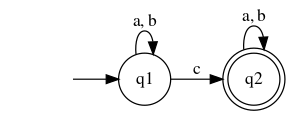
\includegraphics[scale=0.7]{graph1_1.png}
\end{center}

\subsection{}
$$L = \{w \in \{a,b\}^* | |w|_a \leq 2, |w|_b \geq 2 \}$$
\begin{center}
    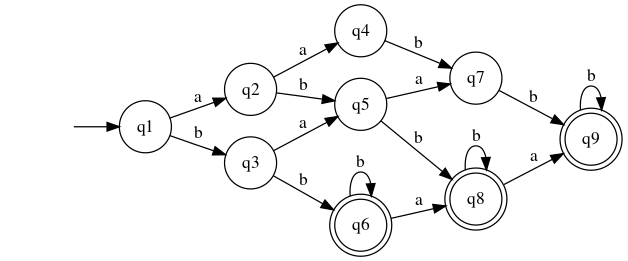
\includegraphics[scale=0.7]{graph1_2.png}
\end{center}

\subsection{}
$$L = \{w \in \{a,b\}^* | |w|_a \neq |w|_b \}$$
Для такого языка невозможно построить КА, так как необходимо считывать количество символов a и b. Поэтому построим для языка, в котором символы чередуются.
\begin{center}
    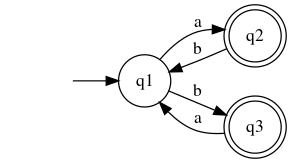
\includegraphics[scale=0.7]{graph1_3.png}
\end{center}

\subsection{}
$$L = \{w \in \{a,b\}^* | ww = www \}$$
\begin{center}
    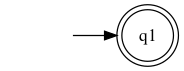
\includegraphics[scale=0.7]{graph1_4.png}
\end{center}
\newpage

% 2
\section{Построить конечный автомат, используя прямое произведение}
Ответом на данное задание является конечный автомат, распознающий описанный язык. Требуется, чтобы он был построен при помощи прямого произведения ДКА и его свойств.

\subsection{}
$$L_1 = \{ w \in \{a,b\}^* | |w|_a \geq 2 \land |w|_b \geq 2\}$$

$$L_{11} = \{ w \in \{a,b\}^* | |w|_a \geq 2 \}$$
$$A_{11} = (\Sigma_1 = \{a, b\}, Q_1 = \{s_1, q_1, t_1\}, s_1, T_1 = \{t_1\}, \delta_1)$$
\begin{center}
    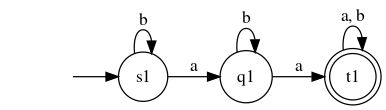
\includegraphics[scale=0.7]{graph2_11.png}
\end{center}

$$L_{12} = \{ w \in \{a,b\}^* | |w|_b \geq 2 \}$$
$$A_{12} = (\Sigma_2 = \{a, b\}, Q_2 = \{s_2, q_2, t_2\}, s_2, T_2 = \{t_2\}, \delta_2)$$
\begin{center}
    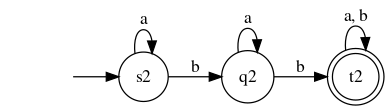
\includegraphics[scale=0.7]{graph2_12.png}
\end{center}
Построим прямое произведение L_1 = L_{11} $\cap$ L_{12}.


$A1 = (\Sigma = \{a, b\}, Q = Q_1 \text{ X } Q_2, s_1s_2, T = \{t_1t_2\}, \delta)$

$Q = \{s_1s_2, s_1q_2, s_1t_2, q_1s_2, q_1q_2, q_1t_2, t_1s_2, t_1q_2, t_1t_2\}$

Зададим функцию перехода $\delta\\$
\nointend
$\delta(s_1s_2, a) = <\delta_1(s_1, a), \delta_2(s_2, a)> = q_1s_2 \hfill \delta(s_1s_2, b) = <\delta_1(s_1, b), \delta_2(s_2, b)> = s_1q_2\\$
$\delta(s_1q_2, a) = q_1q_2 \hfill \delta(s_1q_2, b) = s_1t_2\\$
$\delta(s_1t_2, a) = q_1t_2 \hfill \delta(s_1t_2, b) = s_1t_2\\$
$\delta(q_1s_2, a) = t_1s_2 \hfill \delta(q_1s_2, b) = q_1q_2\\$
$\delta(q_1q_2, a) = t_1q_2 \hfill \delta(q_1q_2, b) = q_1t_2\\$
$\delta(q_1t_2, a) = t_1t_2 \hfill \delta(q_1t_2, b) = q_1t_2\\$
$\delta(t_1s_2, a) = t_1s_2 \hfill \delta(t_1s_2, b) = t_1q_2\\$
$\delta(t_1q_2, a) = t_1q_2 \hfill \delta(t_1q_2, b) = t_1t_2\\$
$\delta(t_1t_2, a) = t_1t_2 \hfill \delta(t_1t_2, b) = t_1t_2\\$

\begin{center}
    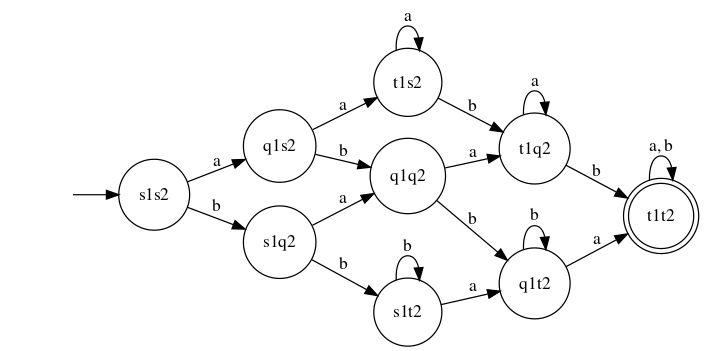
\includegraphics[scale=0.7]{graph2_1.png}
\end{center}


\subsection{}
$$L_2 = \{ w \in \{a,b\}^* | |w| \geq 3 \land |w| \text{ нечетное} \}$$

$$L_{21} = \{ w \in \{a,b\}^* | |w| \geq 3 \}$$
$$A_{21} = (\Sigma_1 = \{a, b\}, Q_1 = \{s_1, q_{11}, q_{12}, t_1\}, s_1, T_1 = \{t_1\}, \delta_1)$$
\begin{center}
    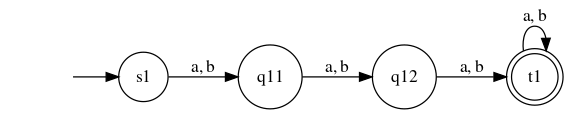
\includegraphics[scale=0.7]{graph2_21.png}
\end{center}

$$L_{22} = \{ w \in \{a,b\}^* | |w| \text{ нечетное} \}$$
$$A_{22} = (\Sigma_2 = \{a, b\}, Q_2 = \{s_2, t_2\}, s_2, T_2 = \{t_2\}, \delta_2)$$
\begin{center}
    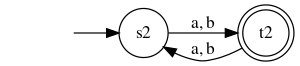
\includegraphics[scale=0.7]{graph2_22.png}
\end{center}
Построим прямое произведение L_2 = L_{21} $\cap$ L_{22}.

$A2 = (\Sigma = \{a, b\}, Q = Q_1 \text{ X } Q_2, s_1s_2, T = \{t_1t_2\}, \delta)$

$Q = \{s_1s_2, s_1t_2, q_{11}s_2, q_{11}t_2, q_{12}s_2, q_{12}t_2, t_1s_2, t_1t_2\}$

Зададим функцию перехода $\delta\\$
\nointend
$\delta(s_1s_2, a) = <\delta_1(s_1, a), \delta_2(s_2, a)> = q_{11}t_2 \hfill \delta(s_1s_2, b) = <\delta_1(s_1, b), \delta_2(s_2, b)> = q_{11}t_2\\$
$\delta(s_1t_2, a) =  q_{11}s_2\hfill \delta(s_1t_2, b) = q_{11}s_2\\$
$\delta(q_{11}s_2, a) =  q_{12}t_2\hfill \delta(q_{11}s_2, b) = q_{12}t_2\\$
$\delta(q_{11}t_2, a) =  q_{12}s_2\hfill \delta(q_{11}t_2, b) = q_{12}s_2\\$
$\delta(q_{12}s_2, a) =  t_1t_2\hfill \delta(q_{12}s_2, b) = t_1t_2\\$
$\delta(q_{12}t_2, a) =  t_1s_2\hfill \delta(q_{12}t_2, b) = t_1s_2\\$
$\delta(t_1s_2, a) =  t_1t_2\hfill \delta(t_1s_2, b) = t_1t_2\\$
$\delta(t_1t_2, a) =  t_1s_2\hfill \delta(t_1t_2, b) = t_1s_2\\$

\begin{center}
    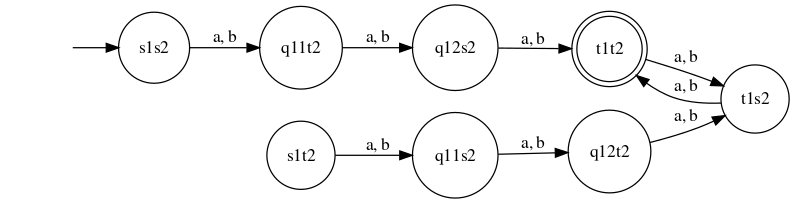
\includegraphics[scale=0.6]{graph2_2.png}
\end{center}
Мы не можем попасть в вершину $s_1t_2$, поэтому убераем нижнию цепь.
\begin{center}
    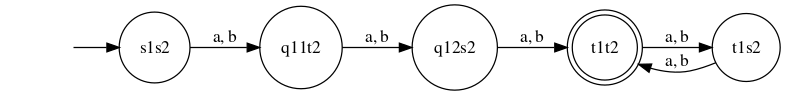
\includegraphics[scale=0.6]{graph2_2'.png}
\end{center}

\subsection{}
$$L_3 = \{ w \in \{a,b\}^* | |w|_a \text{ четно} \land |w|_b \text{ кратно трем} \}$$
$$L_{31} = \{ w \in \{a,b\}^* | |w| \text{ четно} \}$$
$$A_{31} = (\Sigma_1 = \{a, b\}, Q_1 = \{s_1, q_1\}, s_1, T_1 = \{s_1\}, \delta_1)$$
\begin{center}
    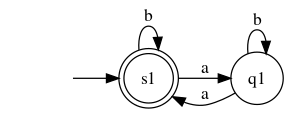
\includegraphics[scale=0.7]{graph2_31.png}
\end{center}

$$L_{32} = \{ w \in \{a,b\}^* | |w|_b \text{ кратно трем} \}$$
$$A_{32} = (\Sigma_2 = \{a, b\}, Q_2 = \{s_2, q21, q22\}, s_2, T_2 = \{s_2\}, \delta_2)$$
\begin{center}
    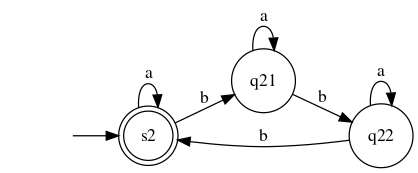
\includegraphics[scale=0.7]{graph2_32.png}
\end{center}
Построим прямое произведение L_3 = L_{31} $\cap$ L_{32}.

$A3 = (\Sigma = \{a, b\}, Q = Q_1 \text{ X } Q_2, s_1s_2, T = \{s_1s_2\}, \delta)$

$Q = \{s_1s_2, s_1q_{21}, s_1q_{22}, q_1s_2, q_1q_{21}, q_1q_{22}\}$

Зададим функцию перехода $\delta\\$
\nointend
$\delta(s_1s_2, a) = <\delta_1(s_1, a), \delta_2(s_2, a)> = q_1s_2 \hfill \delta(s_1s_2, b) = <\delta_1(s_1, b), \delta_2(s_2, b)> = s_1q_{21}\\$
$\delta(s_1q_{21}, a) =  q_1q_{21}\hfill \delta(s_1q_{21}, b) = s_1q_{22}\\$
$\delta(s_1q_{22}, a) =  q_1q_{22}\hfill \delta(s_1q_{22}, b) = s_1s_2\\$
$\delta(q_1s_2, a) =  s_1s_2\hfill \delta(q_1s_2, b) = q_1q_{21}\\$
$\delta(q_1q_{21}, a) =  s_1q_{21}\hfill \delta(q_1q_{21}, b) = q_1q_{22}\\$
$\delta(q_1q_{22}, a) =  s_1q_{22}\hfill \delta(q_1q_{22}, b) = q_1s_2\\$

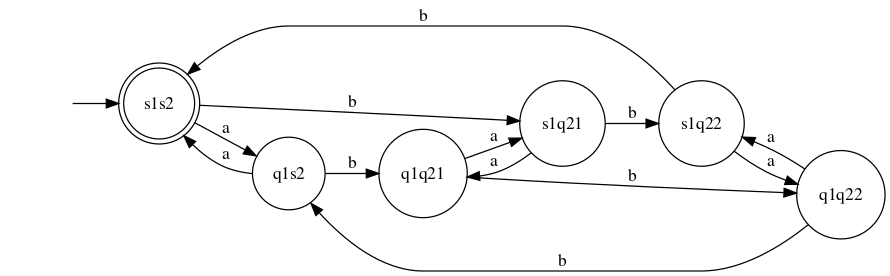
\includegraphics[scale=0.5]{graph2_3.png}

\subsection{}
$$L_4 = \overline{L_3}$$
Автомат остается тем же, изменяются только конечные вершины.


$A_4 = (\Sigma = \{a, b\}, Q = Q_1 \text{ X } Q_2, s_1s_2, T = Q_{prev} \backslash T_{prev}, \delta)\\$
$Q = \{s_1s_2, s_1q_{21}, s_1q_{22}, q_1s_2, q_1q_{21}, q_1q_{22}\}\\$
$T = \{ s_1q_{21}, s_1q_{22}, q_1s_2, q_1q_{21}, q_1q_{22}\}$
\begin{center}
    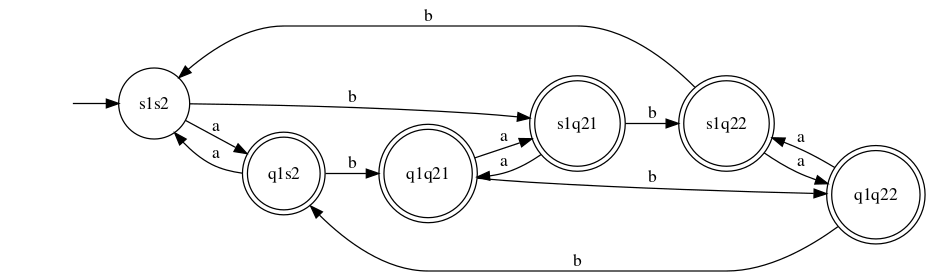
\includegraphics[scale=0.5]{graph2_4.png}
\end{center}


\subsection{}
$$L_5 = L_2 \backslash L_3$$
$L_5 = L_2 \cap \overline{L_3} = L_2 \cap L_4\\$

Упростим ДКА и введем новую нумерацию.
$$A_{51} = (\Sigma_1 = \{a, b\}, Q_1 = \{s_1, q_1, q_2, t_1\}, s_1, T_1 = \{t_1\}, \delta_1)$$
\begin{center}
    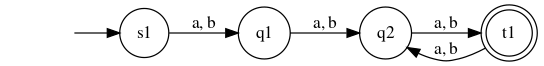
\includegraphics[scale=0.7]{graph2_51.png}
\end{center}
$$A_{52} = (\Sigma_2 = \{a, b\}, Q_2 = \{s_2, p_1, p_2, p_3, p_4, p_5\}, s_2, T_2 = \{p_1, p_2, p_3, p_4, p_5\}, \delta_2)$$
\begin{center}
    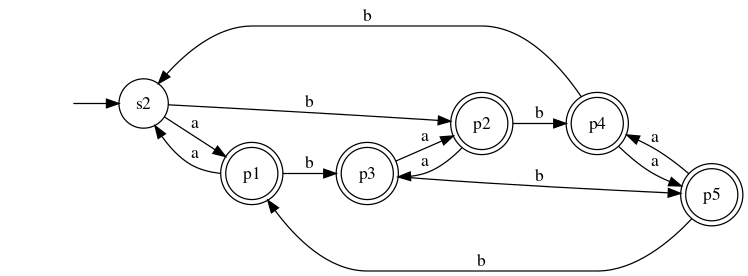
\includegraphics[scale=0.6]{graph2_52.png}
\end{center}
$A_5 = (\Sigma = \{a, b\}, Q = Q_1 \text{ X } Q_2, s_1s_2, T = T_1 \text{ X } T_2, \delta)\\$

$Q = \{ s_1s_2, s_1p_1, s_1p_2, s_1p_3, s_1p_4, s_1p_5, \\
q_1s_2, q_1p_1, q_1p_2, q_1p_3, q_1p_4, q_1p_5, \\
q_2s_2, q_2p_1, q_2p_2, q_2p_3, q_2p_4, q_2p_5, \\
t_1s_2, t_1p_1, t_1p_2, t_1p_3, t_1p_4, t_1p_5\}\\$
$T = \{ t_1s_2, t_1p_1, t_1p_2, t_1p_3, t_1p_4, t_1p_5\}$

Зададим функцию перехода $\delta\\$
\nointend
$\delta(s_1s_2, a) = <\delta_1(s_1, a), \delta_2(s_2, a)> = q_1p_1 \hfill \delta(s_1s_2, b) = <\delta_1(s_1, b), \delta_2(s_2, b)> = q_1p_2\\$
$\delta(s_1p_1, a) = q_1s_2 \hfill \delta(s_1p_1, b) = q_1p_3\\$
$\delta(s_1p_2, a) = q_1p_3 \hfill \delta(s_1p_2, b) = q_1p_4\\$
$\delta(s_1p_3, a) = q_1p_2 \hfill \delta(s_1p_3, b) = q_1p_5\\$
$\delta(s_1p_4, a) = q_1p_5 \hfill \delta(s_1p_4, b) = q_1s_2\\$
$\delta(s_1p_5, a) = q_1p_4 \hfill \delta(s_1p_5, b) = q_1p_1\\$
$\delta(q_1s_2, a) = q_2p_1 \hfill \delta(q_1s_2, b) = q_2p_2\\$
$\delta(q_1p_1, a) = q_2s_2 \hfill \delta(q_1p_1, b) = q_2p_3\\$
$\delta(q_1p_2, a) = q_2p_3 \hfill \delta(q_1p_2, b) = q_2p_4\\$
$\delta(q_1p_3, a) = q_2p_2 \hfill \delta(q_1p_3, b) = q_2p_5\\$
$\delta(q_1p_4, a) = q_2p_5 \hfill \delta(q_1p_4, b) = q_2s_2\\$
$\delta(q_1p_5, a) = q_2p_4 \hfill \delta(q_1p_5, b) = q_2p_1\\$
$\delta(q_2s_2, a) = t_1p_1 \hfill \delta(q_2s_2, b) = t_1p_2\\$
$\delta(q_2p_1, a) = t_1s_2 \hfill \delta(q_2p_1, b) = t_1p_3\\$
$\delta(q_2p_2, a) = t_1p_3 \hfill \delta(q_2p_2, b) = t_1p_4\\$
$\delta(q_2p_3, a) = t_1p_2 \hfill \delta(q_2p_3, b) = t_1p_5\\$
$\delta(q_2p_4, a) = t_1p_5 \hfill \delta(q_2p_4, b) = t_1s_2\\$
$\delta(q_2p_5, a) = t_1p_4 \hfill \delta(q_2p_5, b) = t_1p_1\\$
$\delta(t_1s_2, a) = q_2p_1 \hfill \delta(t_1s_2, b) = q_2p_2\\$
$\delta(t_1p_1, a) = q_2s_2 \hfill \delta(t_1p_1, b) = q_2p_3\\$
$\delta(t_1p_2, a) = q_2p_3 \hfill \delta(t_1p_2, b) = q_2p_4\\$
$\delta(t_1p_3, a) = q_2p_2 \hfill \delta(t_1p_3, b) = q_2p_5\\$
$\delta(t_1p_4, a) = q_2p_5 \hfill \delta(t_1p_4, b) = q_2s_2\\$
$\delta(t_1p_5, a) = q_2p_4 \hfill \delta(t_1p_5, b) = q_2p_1\\$

\begin{center}
    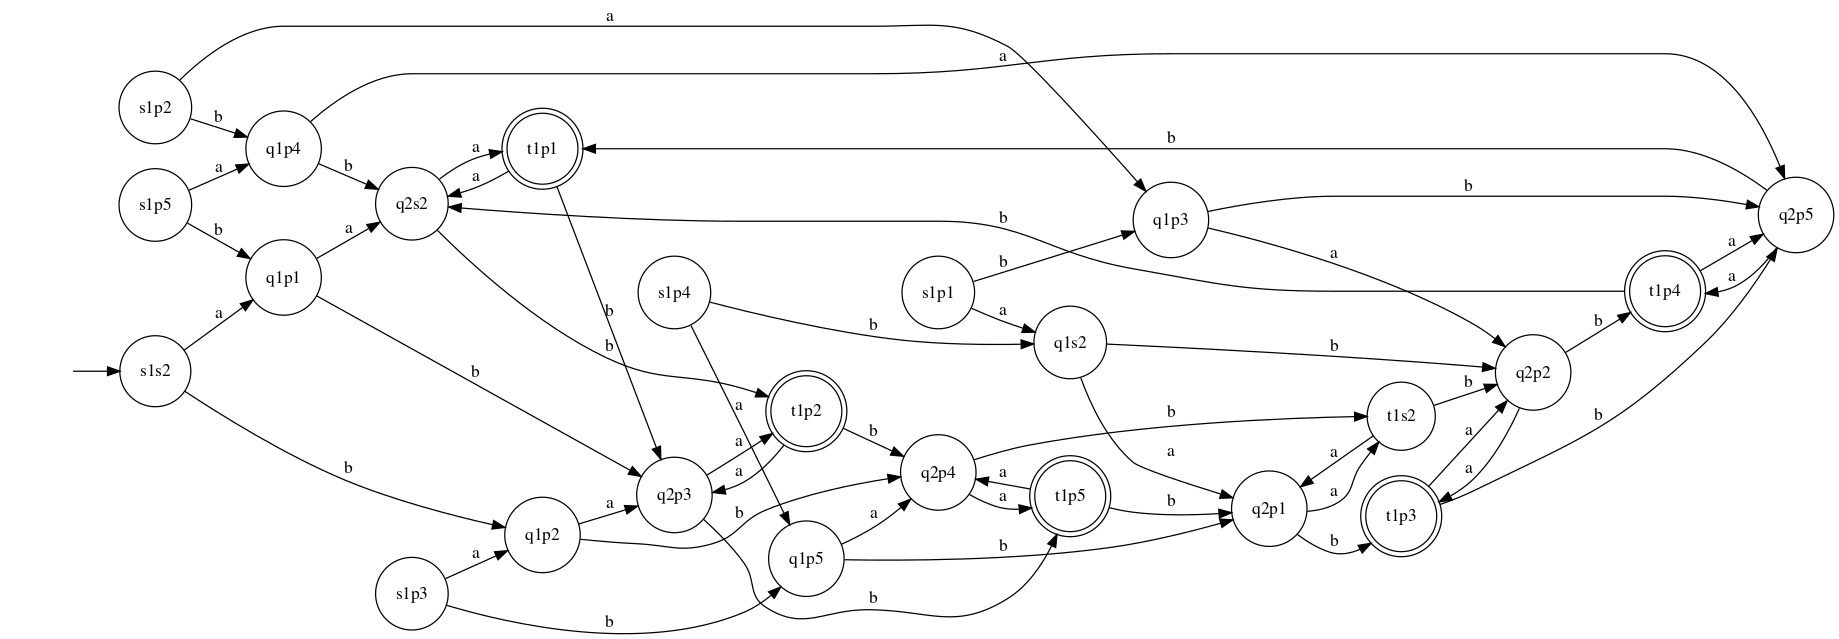
\includegraphics[scale=0.25]{graph2_5.png}
\end{center}

\newpage
% 3
\section{Построить минимальный ДКА по регулярному выражению}
Ответом на данное задание является минимальный ДКА, который допускает тот же язык, что описывается регулярным выражением.

\subsection{}
$$(ab + aba)^*$$

\subsection{}
$$a(a(ab)^*b)^*(ab)^*$$

\subsection{}
$$(a + (a + b)(a + b)b)^*$$

\subsection{}
$$(b + c)((ab)^*c + (ba)^*)^*$$

\subsection{}
$$(a + b)^+(aa + bb + abab + baba)(a + b)^+$$
\newpage

% 4
\section{Определить является ли язык регулярным или нет}
Ответом на данное задание является конечный автомат, если язык регулярен, либо доказательство нерегулярности языка при помощи леммы о разрастании.

\subsection{}
$$L = \{(aab)^nb(aba)^m | n \geq 0, m \geq 0\}$$

\subsection{}
$$L = \{uaav | u \in \{a,b\}^*, v \in \{a,b\}^*, |u|_b \geq |v|_a\}$$

\subsection{}
$$L = \{a^mw | w \in \{a, b\}^*, 1 \leq |w|_b \leq m  \}$$

\subsection{}
$$L = \{ a^kb^ma^n | k = n \lor m > 0\}$$

\subsection{}
$$L = \{ ucv | u \in \{a,b\}^*, v \in \{a,b\}^*, u \neq v^R \}$$
\newpage


% 5
\section{Реализовать алгоритмы}
Ответом на данное задание является работающая программа на выбранном языке программирования, покрытая юнит-тестами.

В рамках своего выполнения программа должна генерировать текстовый документ с картинками, показывающий процесс построения автомата (к примеру, Markdown с графиками на Graphviz).\\
1. Построение ДКА по НКА с $\lambda$-переходами \\
2. Прямое произведение языков, с возможностью построить пересечение, объединение и разность.

\end{document}
